\documentclass[12pt, twoside]{article}
\usepackage[letterpaper, margin=1in, headsep=0.5in]{geometry}
\usepackage[english]{babel}
\usepackage[utf8]{inputenc}
\usepackage{amsmath}
\usepackage{amsfonts}
\usepackage{amssymb}
\usepackage{tikz}
%\usetikzlibrary{quotes, angles}

\usepackage{graphicx}
\usepackage{enumitem}
\usepackage{multicol}

\usepackage{fancyhdr}
\pagestyle{fancy}
\fancyhf{}
\renewcommand{\headrulewidth}{0pt} % disable the underline of the header

\usepackage{setspace}
%\linespread{1.75}

%\fancyhead[RE]{\thepage}
\fancyhead[R]{\thepage \\ Name: \hspace{3cm}}
\fancyhead[L]{BECA / Dr. Huson / 12.1 IB Math SL\\* 4 March 2019}

\begin{document}
\subsubsection*{Unit 5 Exam Part 2: Integral Calculus - without calculator}
 \begin{enumerate}

\subsubsection*{55 minutes. You may \emph{NOT} use a calculator on these problems \hfill [47 marks]}

%\setstretch{1.5}

\item Let $f'(x)=6x^2-5$. Given that $f(2)=-3$, find $f(x)$. \hfill [6]

\item Given $f(2)=2$, $g(2)=-2$, $f'(2)=-1$, and $g'(2)=3$
\begin{enumerate}
    \item Find the derivative of $f+g$ for $x=2$. \hfill [2]
    \item Find the derivative of $f \times g$ for $x=2$. \hfill [2]
    \item Find the derivative of $f \div g$ for $x=2$. \hfill [2]
\end{enumerate}

\item Let $f(x)=x^2$.
  \begin{enumerate}
    \item Find $\int_1^2 (f(x))^2 \,\mathrm{d}x$ \hfill [4]
    \item The following diagram shows part of the graph of $f$.
      \begin{center}
        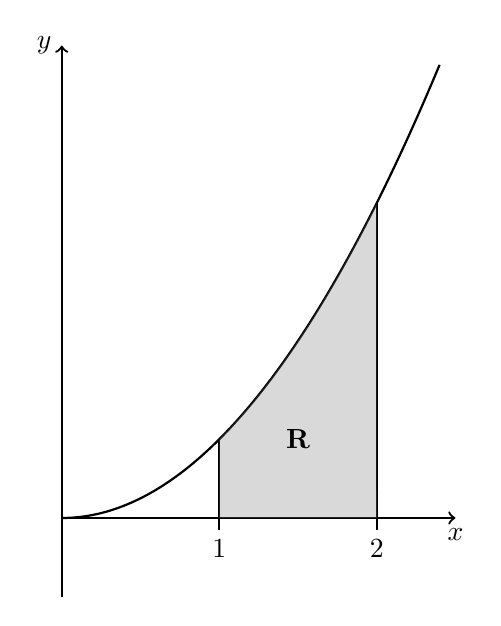
\begin{tikzpicture}[xscale=2,yscale=1]
          \draw [thick, ->] (0,0) -- (2.5,0) node [below] {$x$};
          \draw [thick, ->] (0,-1) -- (0,6) node [left] {$y$};
          \draw[thick, domain=0:2.4] plot[samples=100](\x, {(\x)^2});
          \draw[thick] (1, -.15)node[below]{$1$} --(1,1);
          \draw[thick] (2, -.15)node[below]{$2$} --(2,4);
          \fill[gray,opacity=.3] (1,0)--plot[domain=1:2](\x, {\x*\x})--(2,0);
          \draw (1.5,1) node {$\mathbf{R}$};
        \end{tikzpicture}
      \end{center}
    The shaded region $R$ is enclosed by the graph of $f$, the $x$-axis, and the lines $x=1$ and $x=2$.\\
    Find the volume of the solid formed when $R$ is revolved $360^\circ$ about the $x$-axis.  \hfill [2]
  \end{enumerate}

\item
\begin{enumerate}
    \item Find $\displaystyle \int \frac{1}{2x+3} \,\mathrm{d}x$. \hfill [2]
    \item Given $\displaystyle \int_0^3 \frac{1}{2x+3} \,\mathrm{d}x =\ln \sqrt{P}$, find $P$. \hfill [4]
\end{enumerate}


\newpage
\item The graph of $f(x)=\sqrt{16-4x^2}$, for $-2 \leq x \leq 2$, is shown below.
  \begin{enumerate}
    \item The following diagram shows part of the graph of $f$.
      \begin{center}
        \begin{tikzpicture}[xscale=1.5,yscale=0.75]
          \draw [thick, ->] (-3,0) -- (3.5,0) node [below] {$x$};
          \draw [thick, ->] (0,-3) -- (0,5.5) node [left] {$y$};
            \foreach \x in {-3,..., 3}
            \draw[shift={(\x,0)},color=black] (0pt,-3pt) -- (0pt,0pt) node[below=4pt]  {$\x$};
            \foreach \y in {-3,-2,...,5}
            \draw[shift={(0,\y)},color=black] (-3pt,0pt) -- (0pt,0pt) node[left=3pt]  {$\y$};
          \draw[thick, domain=-2:2] plot[samples=100](\x, {(16-4*(\x)^2)^0.5});
        \end{tikzpicture}
      \end{center}
    The region enclosed by the curve of $f$ and the $x$-axis is rotated $360^\circ$ about the $x$-axis.\\
    Find the volume of the solid formed.  \hfill [6]
  \end{enumerate}


\item Let $f(x)=\sqrt{x}$. Line $L$ is the normal to the graph of $f$ at the point $(4,2)$.
  \begin{enumerate}
    \item Show that the equation of $L$ is $y=-4x+18$. \hfill [4]
    \item Point $A$ is the $x$-intercept of $L$. Find the $x$-coordinate of $A$. \hfill [2]
    \item In the diagram below, the shaded region $R$ is bounded by the $x$-axis, the graph of $f$, and the line $L$.
      \begin{center}
        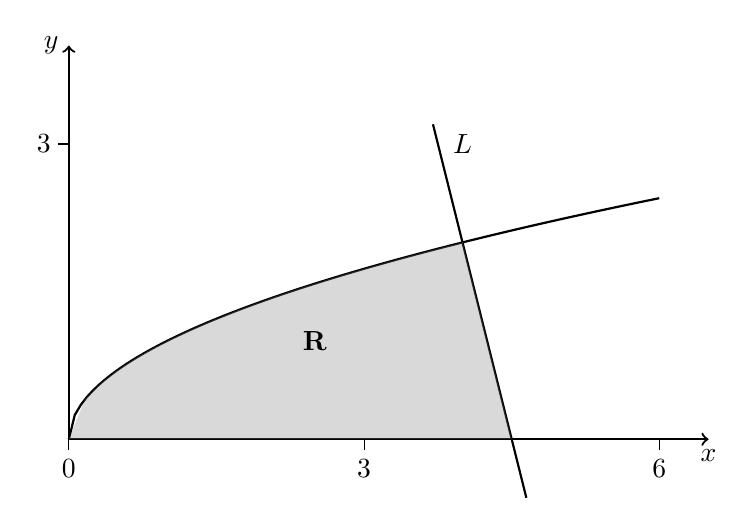
\begin{tikzpicture}[xscale=1.25,yscale=1.25]
          \draw [thick, ->] (0,0) -- (6.5,0) node [below] {$x$};
          \draw [thick, ->] (0,0) -- (0,4) node [left] {$y$};
            \foreach \x in {0, 3, 6}
            \draw[shift={(\x,0)},color=black] (0pt,-3pt) -- (0pt,0pt) node[below=4pt]  {$\x$};
            \foreach \y in {3}
            \draw[shift={(0,\y)},color=black] (-3pt,0pt) -- (0pt,0pt) node[left=3pt]  {$\y$};
          \draw[thick, domain=0:6] plot[samples=100](\x, {(\x)^0.5});
          \draw[thick, domain=3.7:4.65] plot[samples=100](\x, {-4*(\x)+18});
          \fill[gray,opacity=.3] (0,0)--plot[domain=0:4](\x, {(\x)^0.5})--(4.5,0);
          \draw (2.5,1) node {$\mathbf{R}$};
          \draw (4,3) node {$L$};
        \end{tikzpicture}
      \end{center}
      Find and expression for the area of $R$.  \hfill [3]
    \item The region $R$ is rotated $360^\circ$ about the $x$-axis. Find the volume of the solid formed, giving your answer in terms of $\pi$.  \hfill [8]
  \end{enumerate}



\end{enumerate}
\end{document}
